\chapter*{Introducción}

\emph{Deep Learning} is the branch inside \emph{machine learning} which allows to design non-linear algebra models \cite{dl-nature}.


Para la parte que nos atañe, podemos realizar una división funcional en las dos principales funciones que realizan los algoritmos de \emph{machine learning} aplicados a procesamiento de imagen:

\begin{itemize}
	\item \textbf{Clasificación:} dado un conjunto $\{c_1, c_2, ..., c_n\}$ de posibles clases a las que una imagen $x_i$ puede pertenecer, seleccionar la clase $c_i$ a la que más probablemente se ajustará $x_i$, dado un conjunto determinado de características.
	\item \textbf{Detección}: dada una imagen $x_i$, decidir si dentro de la misma podemos encontrar un objeto y/o región que se amolde al tipo buscado (\emph{e.g.} persona, perro, etc.) y, en caso afirmativo, localizarlo (ya sea mediante una región o mediante una caja (\emph{bounding box}).
\end{itemize}

\begin{figure}[h]
	\centering
	\begin{subfigure}[h!]{0.6\textwidth}
		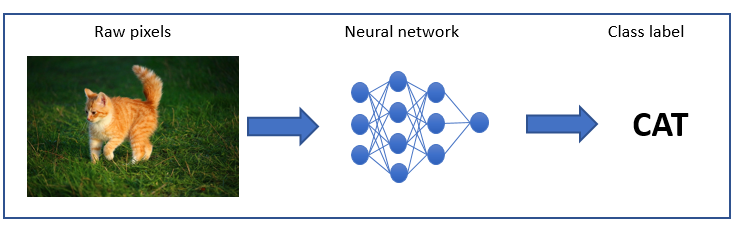
\includegraphics[width=\textwidth]{images/classification}
		\caption{Clasificación (imagen de esciencecenter.nl REF)}
		\label{fig:1_classification}
	\end{subfigure}
	
	\qquad
	
	\begin{subfigure}[h!]{0.6\textwidth}
		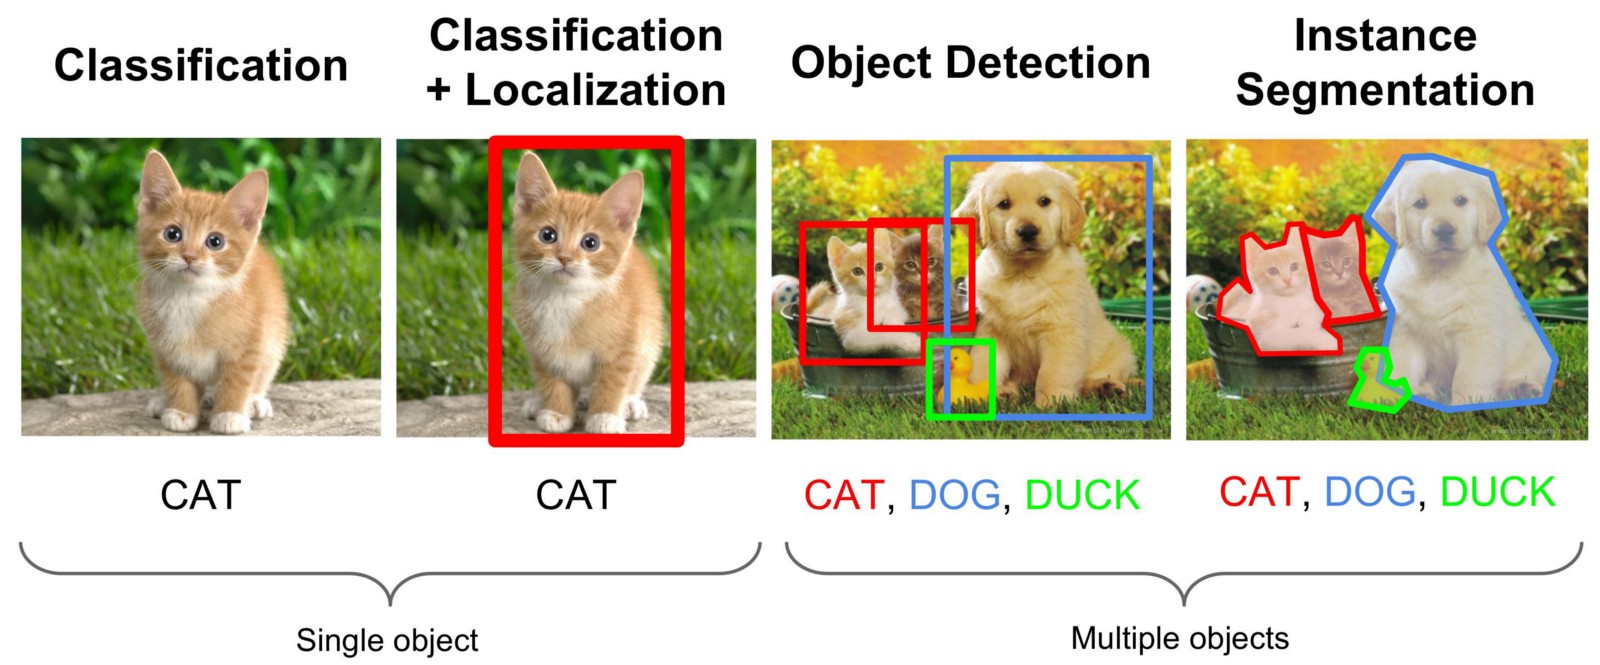
\includegraphics[width=\textwidth]{images/detection}
		\caption{Detección (imagen de medium.com REF)}
		\label{fig:1_detection}			
	\end{subfigure}
	
	\caption{Diferencia funcional entre clasificación y detección.}
	\label{fig:1_class_vs_det}
\end{figure}



